

\begin{center}
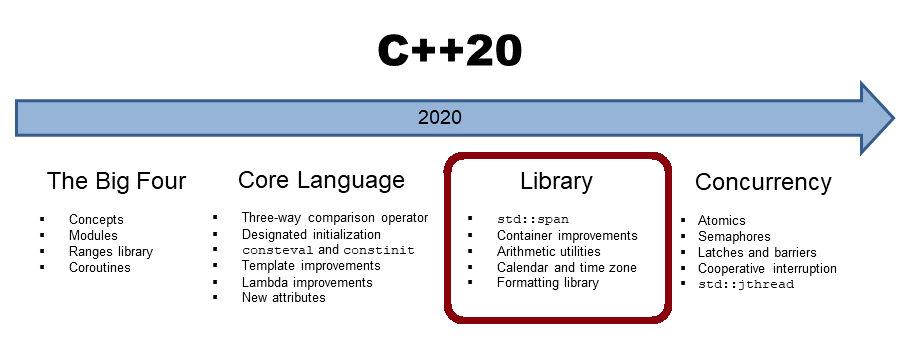
\includegraphics[width=1.0\textwidth]{content/2/chapter3/images/6.png}\\
\end{center}

\subsubsubsection{3.3.1\hspace{0.2cm}std::span}

std::span表示引用一个连续的序列,有时也称为视图,并不是数据的所有者。视图可以是一个C风格数组,一个std::array,一个有长度的指针,或者一个std::vector。std::span的实现需要指向其第一个元素的指针和长度。使用std::span的主要原因是,若将普通数组传递给函数,数组会衰退为指针,其长度信息会丢失。std::span可以自动推导数组、std::array或Std::vector的长度。若使用指针初始化std::span,则必须在构造函数中提供其长度。

\hspace*{\fill} \\ %插入空行
\noindent
\textbf{std::span作为函数参数}
\begin{lstlisting}[style=styleCXX]
void copy_n(const int* src, int* des, int n){}

void copy(std::span<const int> src, std::span<int> des){}

int main(){
	
	int arr1[] = {1, 2, 3};
	int arr2[] = {3, 4, 5};
	
	copy_n(arr1, arr2, 3);
	copy(arr1, arr2);
	
}
\end{lstlisting}

与函数copy\_n相比,copy不需要元素的数量。因此,std::span<T>是导致错误的常见原因。

\subsubsubsection{3.3.2\hspace{0.2cm}容器的改进}

C++20在标准模板库的容器方面有很多改进。首先,std::vector和std::string具有constexpr构造函数,因此可以在编译时使用。所有标准库容器都支持擦除,关联容器支持contains成员函数。此外,std::string允许检查前缀或后缀。

\subsubsubsection{3.3.3\hspace{0.2cm}计算工具}

有时,有符号整数和无符号整数的比较是导致意外行为和错误的原因,新的安全整数比较函数std::cmp\_*可以避免这种问题。

\hspace*{\fill} \\ %插入空行
\noindent
\textbf{安全的整数比较}
\begin{lstlisting}[style=styleCXX]
int x = -3;
unsigned int y = 7;

if (x < y) std::cout << "expected";
else std::cout << "not expected"; // not expected

if (std::cmp_less(x, y)) std::cout << "expected"; // expected
else std::cout << "not expected";
\end{lstlisting}

此外,C++20在命名空间std::numbers中包含了数学常量,包括e、π和φ。

新的位操作允许访问单个位和位序列,并重新解释它们。

\hspace*{\fill} \\ %插入空行
\noindent
\textbf{访问单个位和位序列}
\begin{lstlisting}[style=styleCXX]
std::uint8_t num= 0b10110010;

std::cout << std::has_single_bit(num) << '\n'; // false
std::cout << std::bit_width(unsigned(5)) << '\n'; // 3
std::cout << std::bitset<8>(std::rotl(num, 2)) << '\n'; // 11001010
std::cout << std::bitset<8>(std::rotr(num, 2)) << '\n'; // 10101100
\end{lstlisting}

\subsubsubsection{3.3.4\hspace{0.2cm}格式化库}

新的格式化库提供了更安全且可扩展的替代方案,旨在补充现有的I/O流,并重用其一些基础结构,例如:用于定义类型的重载插入操作符。

\begin{lstlisting}[style=styleCXX]
std::string message = std::format("The answer is {}.", 42);
\end{lstlisting}

std::format使用Python的语法进行格式化。下面的例子展示了一些用例:

\begin{itemize}
\item 
格式和使用位置参数

\begin{lstlisting}[style=styleCXX]
std::string s = std::format("I'd rather be {1} than {0}.", "right", "happy");
// s == "I'd rather be happy than right."
\end{lstlisting}

\item 
以安全的方式将整数转换为字符串

\begin{lstlisting}[style=styleCXX]
memory_buffer buf;
std::format_to(buf, "{}", 42); // replaces itoa(42, buffer, 10)
std::format_to(buf, "{:x}", 42); // replaces itoa(42, buffer, 16)
\end{lstlisting}

\item 
格式化用户定义的类型

\end{itemize}

\subsubsubsection{3.3.5\hspace{0.2cm}日期和时区}

C++11中的\href{https://en.cppreference.com/w/cpp/chrono}{chrono库}扩展了日期和时区功能。日期由表示年、月、周中的天和月中的第n个工作日组成。这些基本类型可以组合,形成复杂类型,例如:year\_month、year\_month\_day、year\_month\_day\_last、year\_month\_weekday和year\_month\_weekday\_last。为了方便地指定时间点,操作符“/”可以重载。此外,可以用新字面量: d表示天,y表示年。

时间点可以显示在不同的时区。由于扩展了chrono库,下面的用例实现起来就很简单:

\begin{itemize}
\item 
以特定格式表示日期

\item 
一个月的最后一天

\item 
获取两个日期之间的天数

\item 
输出不同时区的当前时间
\end{itemize}

下面的程序显示了不同时区的当前时间。

\hspace*{\fill} \\ %插入空行
\noindent
\textbf{不同时区的当前时间}
\begin{lstlisting}[style=styleCXX]
using namespace std::chrono;

auto time = floor<milliseconds>(system_clock::now());
auto localTime = zoned_time<milliseconds>(current_zone(), time);
auto berlinTime = zoned_time<milliseconds>("Europe/Berlin", time);
auto newYorkTime = zoned_time<milliseconds>("America/New_York", time);
auto tokyoTime = zoned_time<milliseconds>("Asia/Tokyo", time);

std::cout << time << '\n'; // 2020-05-23 19:07:20.290
std::cout << localTime << '\n'; // 2020-05-23 21:07:20.290 CEST
std::cout << berlinTime << '\n'; // 2020-05-23 21:07:20.290 CEST
std::cout << newYorkTime << '\n'; // 2020-05-23 15:07:20.290 EDT
std::cout << tokyoTime << '\n'; // 2020-05-24 04:07:20.290 JST
\end{lstlisting}

